\documentclass[12pt,a4,utf8]{article}

% Language setting
% Replace `english' with e.g. `spanish' to change the document language
\usepackage{babel}

% Set page size and margins
% Replace `letterpaper' with`a4paper' for UK/EU standard size
\usepackage[letterpaper,top=2cm,bottom=2cm,left=3cm,right=3cm,marginparwidth=1.75cm]{geometry}

% Useful packages
\usepackage{ctex}
\usepackage{amsmath,amsfonts,amsthm}
\usepackage{bm}
\usepackage{mathrsfs}
\usepackage{graphicx}
\usepackage[colorlinks=true, allcolors=blue]{hyperref}
\usepackage{lmodern}
\usepackage{microtype}
\usepackage{commath}
\usepackage{caption}
\usepackage{cite}
\usepackage{subfigure}
\usepackage[numbers,sort&compress]{natbib}
\usepackage{booktabs}
\usepackage{array}
\usepackage{epstopdf}
\newcommand{\upcite}[1]{\textsuperscript{\textsuperscript{\cite{#1}}}} % 使得参考文献变为上标


\title{重力补偿惯性导航技术的应用与发展}
\author{胡其秦}
\bibliographystyle{unsrt}
\begin{document}
\maketitle

\begin{abstract}
      XXXXXXX
\end{abstract}

\section{介绍}

向海而兴,向海而强,自15世纪以来,人类就拉开了大航海时代的帷幕。随着科学家们对海洋认识的不断加深,新型航海技术日新月异,世界各国已经不再是一个个被分割的孤岛,而是相互连结的命运共同体。充分开发海洋资源,发展海洋贸易,建设海洋强国,首先是要加快海洋科技创新的步伐。但汪洋无际,复杂多变的海洋环境给航行的船只和舰艇的作业活动带来了许多难题,其中亟需解决的是水下高精度导航定位问题。水下导航的难点不光是在导航定位本身上,更是因为复杂多变的水下环境带来了不小的阻碍,让原本适用于地面的诸多方法失效于水下,比如我们常见的卫星导航,由于水体介质不利于电磁波的传播,所以目前来说在深海区域无法直接接收到有效的卫星信号。而相比之下,惯性导航依托自身的惯性器件测量输出的结果,并不需要其他外来的数据,所以能够保持较高的自主性和无源性,使之成为主要的水下导航方式。然而,惯性导航的定位精度往往与其自身的器件工艺与相应的算法有关,在没有其他参考信息进行误差修正的情况下,只能在短时间内保持一定的导航精度。随着导航解算时间的不断增加,相应的各种误差也将随时间不断积累,如果不能采取及时有效的误差修正手段,惯性导航将无法满足正常的导航精度需求,最终导致其彻底失效。因此,发展以惯导为主、多手段辅助导航系统成为水下导航定位系统的发展方向。

为了能够满足水下导航的正常需求,人们不得不从地球自身的地理特征上寻找方法,比如地形轮廓、地球磁场、地球重力场等。与陆地上不同,因为海下环境的复杂性,以目前的技术手段很难有效的成功提取海底特征;而且由于水下载体自身金属结构的特殊性,加上大量的用电设施,很容易对本就微弱的地球磁场产生进一步的干扰,增大其检测难度。无独有偶,重力场作为一种无源、不交叉重合的地球特征场,由于其只与地球本身有关,短时间内并不会有明显的变化,自上个世纪以来一直成为人们研究的热点,相关领域可以追溯到测绘、地质勘探、天体物理等多个研究方向。更重要的是,在哥式效应的作用下,加速度计和陀螺仪无法区分载体的加速度和重力加速度,而往往重力场的信息是通过正常重力场模型给出,这对于追求高精度的惯性导航来说,成为了制约其发展的重要影响因素之一。目前国际上高精度惯导的指标已经优于1n mail/h\upcite{article},但离水下无源自主导航最终实现“码头到码头(Port-to-Port)”这一目标还有相当长的一段距离\upcite{moryl1997advanced}。因此如何提取出重力扰动并有效地应用于惯导中补偿,是开展重力辅助惯性导航后续研究的关键性步骤,也是其重要前提\upcite{WHCH20240724001}。

\section{重力测量}
      重力测量最早可以追溯到16世纪,1590年伽利略首次利用观测物体自由落体运动的方法测量到了重力加速度。历史上,惠更斯在17世纪推导了摆钟周期$T$与摆长$L$和重力加速度$g$的关系,从而研制出了第一架可以测定重力加速度的摆钟\upcite{snelders1989christiaan},为重力测量奠定了基础。在十九世纪末期,匈牙利物理学家厄缶研制出了扭秤,这标志着重力勘探技术的诞生\upcite{szabo2016history,veryaskin2021gravity}。然而,到了二十世纪三十年代,由于扭秤在测量上耗时较长且易受地形变化的影响,它逐渐被新一代的重力测量设备所替代,这些设备虽灵敏度略低,但测量速度快、稳定性强\upcite{chendaiyong}。

根据测量目标的区别,可以将重力仪分为标量重力仪、矢量重力仪以及重力梯度仪\upcite{schwarz1995some}。标量重力测量通常使用一个精确的垂直加速度计来确定重力场中垂向重力异常,没有提供方向信息;矢量重力仪不仅测量重力异常的大小,还测量其方向,包含垂向和水平方向的重力扰动信息,所以测量结果往往能够更好的反映重力场的空间分布情况,在现在拥有更广泛的应用;重力梯度仪则是测量重力场的空间变化率(即重力势的梯度),在需要解析高频重力信号和高精度重力场研究中,能够提供更高的分辨率和丰富的细节特征,拥有更广阔的应用前景。

根据搭载的平台设备区别,重力测量可以分为地面重力测量、海洋重力测量、航空重力测量和卫星重力测量\upcite{hirt2013new,liang2020high,kwon2001new},表\ref{tab_1}分析了四种方式的优缺点及发展趋势。现代开展海洋重力测量的仪器是海洋重力仪,其中海洋重力测量一般采用静力法相对重力测量。由于海洋重力仪需要安装在动基座(如船舶、潜艇等)进行测量工作,需要面临恶劣海况的干扰,各种有害加速度信息和厄特弗斯效应会影响到重力加速度的测量结果\upcite{ZGZC201808001017}。与传统的船载重力测量手段不同,为了获得更加真实的海洋重力数据,近几年研究人员进一步提出水下移动重力测量,使AUV搭载相关重力测量仪器平台,与母船之间通过拖缆连接实现信息反馈,实现水下移动重力测量实验\upcite{1021532813.nh}。图\ref{fig_2}为国防科技大学研制的水下重力仪搭载“海洋四号”调查船进行的水下重力测量实验。

\begin{figure}[h]
      \centering
      \subfigure[一级拖体]{
            \begin{minipage}{0.45\linewidth}
                  \centering
                  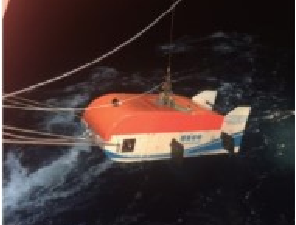
\includegraphics[width=0.9\textwidth]{figure/first_tag-crop.pdf}
                  \captionsetup{font={scriptsize}}
            \end{minipage}
      }
      \subfigure[二级拖体]{
            \begin{minipage}{0.45\linewidth}
                  \centering
                  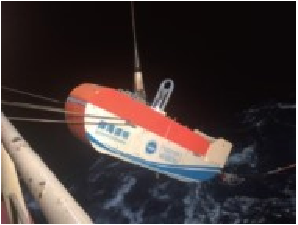
\includegraphics[width=0.9\textwidth]{figure/second_tag-crop.pdf}
            \end{minipage}
      }
      \captionsetup{font={footnotesize}}
      \caption{“海洋四号”科考船实施水下拖拽移动重力测量实验\upcite{DHKZ2020Z1020}}
      \label{fig_2}
\end{figure}

设计的重力仪的平台架构是否稳定,往往决定了其测量的精度,因此更好的平台稳定性是所有新系统开发的主要目标。文献\cite{huang2017development}基于不同的稳定平台方案类型,将当前主流的海空重力仪划分为四种\upcite{huang2017development,lacoste1967lacoste,Zongjie,Reviewon,Newlydeveloped,valliant2019lacoste}:第一种是双轴阻尼陀螺平台,代表性产品包括L$\And$R系列、ZLS型、DGS型、KSS型、BGM型和CHZ型重力仪;第二种是双轴惯导加捷联方位平台,代表性产品包括Chenkan-AM型和GDP型重力仪;第三种是三轴惯导平台,代表性产品包括AirGrav型、GIPS-AM型和GT系列重力仪;第四种是捷联惯导平台,代表性产品包括SISG系统、SAGS系统、SGA-WZ型和SAG型捷联重力仪。
其中,前三种为物理平台,可以有效隔离载体的角运动和振动,因此能够提供更稳定的测量环境,具有较好的长期稳定性和更高的作业效益。捷联式重力仪作为数学平台,不需要水平稳定的平台,结构相对比较简单,可以快速响应载体的姿态变化,便于在各种载体上集成使用;更重要的是,捷联式重力测量对于类似湍流类的扰动敏感性低,即使在强烈的扰动环境中也能够进行重力测量,而更成熟的平台稳定式弹簧重力仪对强湍流相当敏感\upcite{becker2016advanced}。而且研究表明\upcite{johann2019direct,wei1998flight,bastos2002gravity},如果通过消除线性漂移来减少强IMU漂移的影响,则可以实现与使用稳定平台重力仪类似的水平精度。
% Table generated by Excel2LaTeX from sheet 'Sheet1'
\begin{table}[htbp]
      \centering
      \caption{重力测量的基本方法}
        \begin{tabular}{m{6.3em}<{\centering} m{7em}<{\centering} m{7.6em}<{\centering} m{10.125em}<{\centering}}
        \toprule
        \textbf{测量方法} & \multicolumn{1}{c}{\textbf{优点}} & \multicolumn{1}{c}{\textbf{缺点}} & \multicolumn{1}{c}{\textbf{发展趋势}} \\
        \midrule
        地面重力测量 & 精度高,可以提供绝对重力值或详细的重力异常数据 & 效率低,覆盖区域有限,不适合大范围快速测量 & 地面重力测量仪器变得更加轻便和自动化,动态性能和实时性能表现更好,测量效率提高 \\
        \midrule
        海洋重力测量 & 适用于大面积海洋区域的重力场调查 & 受海况影响较大,精度可能受到船体运动和海洋噪声的影响 & 结合卫星遥感技术,提高海洋重力测量的动态性和实时性,精度和稳定性有更好的发展 \\
        \midrule
        航空重力测量 & 覆盖面积广,数据获取速度快,适用于难以到达的地区 & 成本较高,受天气条件限制,精度可能受到飞行高度和速度的影响 & 随着无人机技术的发展,航空重力测量将会更加灵活和经济;\newline{}采集的数据会得到快速处理和实时应用 \\
        \midrule
        卫星重力测量 & 全球覆盖,可以监测到偏远或难以接近的地区 & 空间分辨率较低,受大气和卫星轨道误差的影响 & 卫星重力测量的分辨率和精度会持续提高;\newline{}出现多卫星联合观测的模式,提高全球重力场数据的获取频率和覆盖范围的能力 \\
        \bottomrule
        \end{tabular}%
      \label{tab_1}%
\end{table}%    

\subsection{国外捷联式重力仪研究现状}
上个世纪五六十年代,捷联式重力仪主要以测量标量重力为主\upcite{peshekhonovstate,thompson1959aerial,thompson1960aerial},1958年美国空军首次在加利福尼亚州爱德华兹空军基地上空进行了机载L$\And$R海洋重力仪的第一次测试,并且获得了5分钟平均重力读数,精度优于10mGal。1965年,美国空军将L$\And$R重力仪装配平衡架并搭载在CH-3E直升机上进行位置确定,测量载体高度。随着80年代差分全球定位系统(Differential Global Position System,DGPS)的高速发展,航空重力测量的精度问题逐渐得到解决\upcite{thompson1960aerial,brozena1989interferometric,schwarz1989comparison,kleusberg1990airborne},因此大量的关于捷联式重力仪的相关研究和测试开始展开。以加拿大Calgary大学的基于捷联惯导系统的航空标量重力测量系统(Strapdown Inertial Scalar Gravimetry,SISG)、德国巴伐利亚自然与人文科学学院的SAGS系统、德国iMAR Navigation gmbH(iMAR)系列捷联式重力仪和俄罗斯莫斯科重力测量技术公司的GT-X型重力仪为代表\upcite{bruton2000improving,meyer2003angel,bastos2002gravity,boedecker2006sags4,berzhitskii2010airborne,hoss20201}。
\subsection{国内捷联式重力仪研究现状}
由于种种原因,我国在重力测量领域起步较晚,自1969年以来,先后引进了一批国外制造的海洋重力仪,其中以前西德的产品居多。自21世纪第二个十年以来,中国在重力仪研制领域取得了快速进展。北京航天控制仪器所于2010年开始了平台式和捷联式航空重力仪的研制,SGA型捷联式重力仪和SAG-2M型海洋重力仪在海洋试验中都取得了优于1mGal内符合精度的测试结果\upcite{xiurui}。中国第一台捷联式机载标量重力仪SGA-WZ于2010年在国防科技大学(NUDT)惯性技术实验室研制成功\upcite{DHKZ2020Z1020},并在2012年受邀参加格陵兰岛进行的航空飞行测试。此后,基于丰富的技术及经验,在第一代的基础上持续改进和创新,目前已实现了四代五型捷联式重力仪的研制工作,分别是第二代SGA-WZ02重力仪,基于“捷联+平台”理念的第三代重力仪SGA-WZ03、第三代水下重力仪以及第四代SGA-WZ04和第五代SGA-WZ05捷联式重力仪,目前优于0.6mGal的动态重复测量精度使得其性能达到了国际先进水平。2018年,向阳红6号科考船搭载6个型号的海洋重力仪(CHZ-Ⅱ、SAG-2M、SGA-WZ、ZL11、俄罗斯GT-2M和美国LCR)在南海海域开展对比试验,试验结果表明,国产重力仪精度接近GT-2M重力仪,高于LCR重力仪\upcite{yuan2020performance}。

在为我国重力仪研制工作取得重大突破而感到鼓舞的同时,也应该清楚地认识到与西方发达国家之间的差距。特别是重力仪作为各国之间重要的战略型武器,我们国家如何在保持独立自主、自立根生的同时,打破信息封锁、紧跟世界前沿,需要所有的科技工作者共同努力。

\section{重力扰动定义及测量方法}
\subsection{定义}
假设地球可以被近似为一个绕其短轴均匀旋转的椭球体,并且这个椭球体的表面是一个等势面,那么正常重力可以用Somigliana公式的泰勒级数展开来计算\upcite{somigliana1929teoria}。但是实际上地球并非一个理想的旋转椭球体,真实的重力与正常重力之间必然会存在一个偏差,如图\ref{fig_1}所示。在图a中$H$代表大地水准面高,$N$代表大地水准面相对于椭球表面的高度,$h_t$代表地形高度。我们通常将真实重力与正常重力之间的差值定义为重力扰动$\bm{\delta g} = \bm{g} - \bm{g}_0$,在东北天坐标系下,重力扰动在正常重力方向下的投影为重力异常$\Delta g = -\delta g_U $,真实重力与正常重力在水平方向的夹角称作垂线偏差,并定义在卯酉圈方向上的分量记为$\eta$,在子午圈方向上的分量记为$\zeta$。当垂线偏差满足小角度条件(即重力扰动水平分量远小于正常重力大小)时,有如下的近似关系
 
\begin{figure}[h]
      \centering
      \subfigure[椭球模型及大地水准面]{
            \begin{minipage}{0.66\linewidth}
                  \centering
                  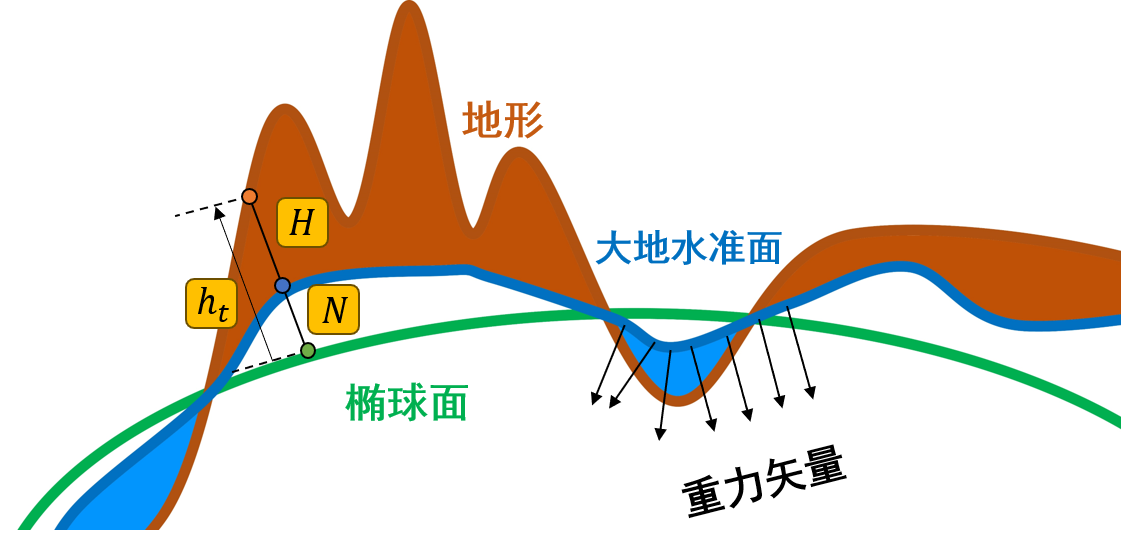
\includegraphics[width=0.9\textwidth]{figure/figure_gdiod.png}
                  \captionsetup{font={scriptsize}}
            \end{minipage}
      }
      \subfigure[重力扰动模型]{
            \begin{minipage}{0.25\linewidth}
            \centering
                  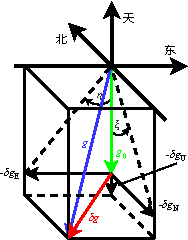
\includegraphics[width=0.9\textwidth]{figure/gra_dis-crop.pdf}
            \end{minipage}
      }
      \captionsetup{font={footnotesize}}
      \caption{\label{fig_1}}
\end{figure}

\begin{equation}
      \begin{aligned}
            \eta & \approx -\delta g_E / \gamma \\
            \xi  & \approx -\delta g_N / \gamma
      \end{aligned}
      \label{equ_1}
\end{equation}

根据几何关系可知,真实重力与正常重力、垂线偏差和重力异常之间的关系为
\begin{equation}
      \begin{aligned}
            \bm{g}^n & = \bm{\gamma}^n + \delta \bm{g}^n               \\
                     & =\begin{bmatrix}
                              0 & 0 & -\gamma
                        \end{bmatrix}^T +
            \begin{bmatrix}
                  \delta g_E & \delta g_N & \delta g_U
            \end{bmatrix}^T                       \\
                     & = \begin{bmatrix}
                               -\gamma\eta & -\gamma\xi & -\gamma - \Delta g
                         \end{bmatrix}^T
      \end{aligned}
      \label{equ_2}
\end{equation}

因此, 对于1arcsec的垂线偏差,大约会产生5mGal的水平重力误差\upcite{jekeli1994airborne},这对于高精度惯导来说,补偿是必要的。

\subsection{测量方法}
在使用捷联式重力仪进行重力扰动的测量中,主要有两种方法进行测量\upcite{jekeli1997gps},分别是直接测量和间接测量。

直接测量就是根据牛顿第二定律,利用测得的物体运动加速度$\bm{\ddot{r}}$减去惯性测量单元(IMU)所测得的比力$\bm{f}$的量作为实测的重力,于是有的文献将其称呼为“加速度计测量法”\upcite{johann2019direct},如式\ref{equ_3}所示
\begin{equation}
      \bm{g} = \bm{\ddot{r}} - \bm{f}
      \label{equ_3}
\end{equation}
其中,物体的运动加速度$\bm{\ddot{r}}$一般通过卫星观测值进行相应的微分处理得到的。进一步的,重力扰动的处理流程如图\ref{fig:direct}所示

\begin{figure}[h]
      \centering
      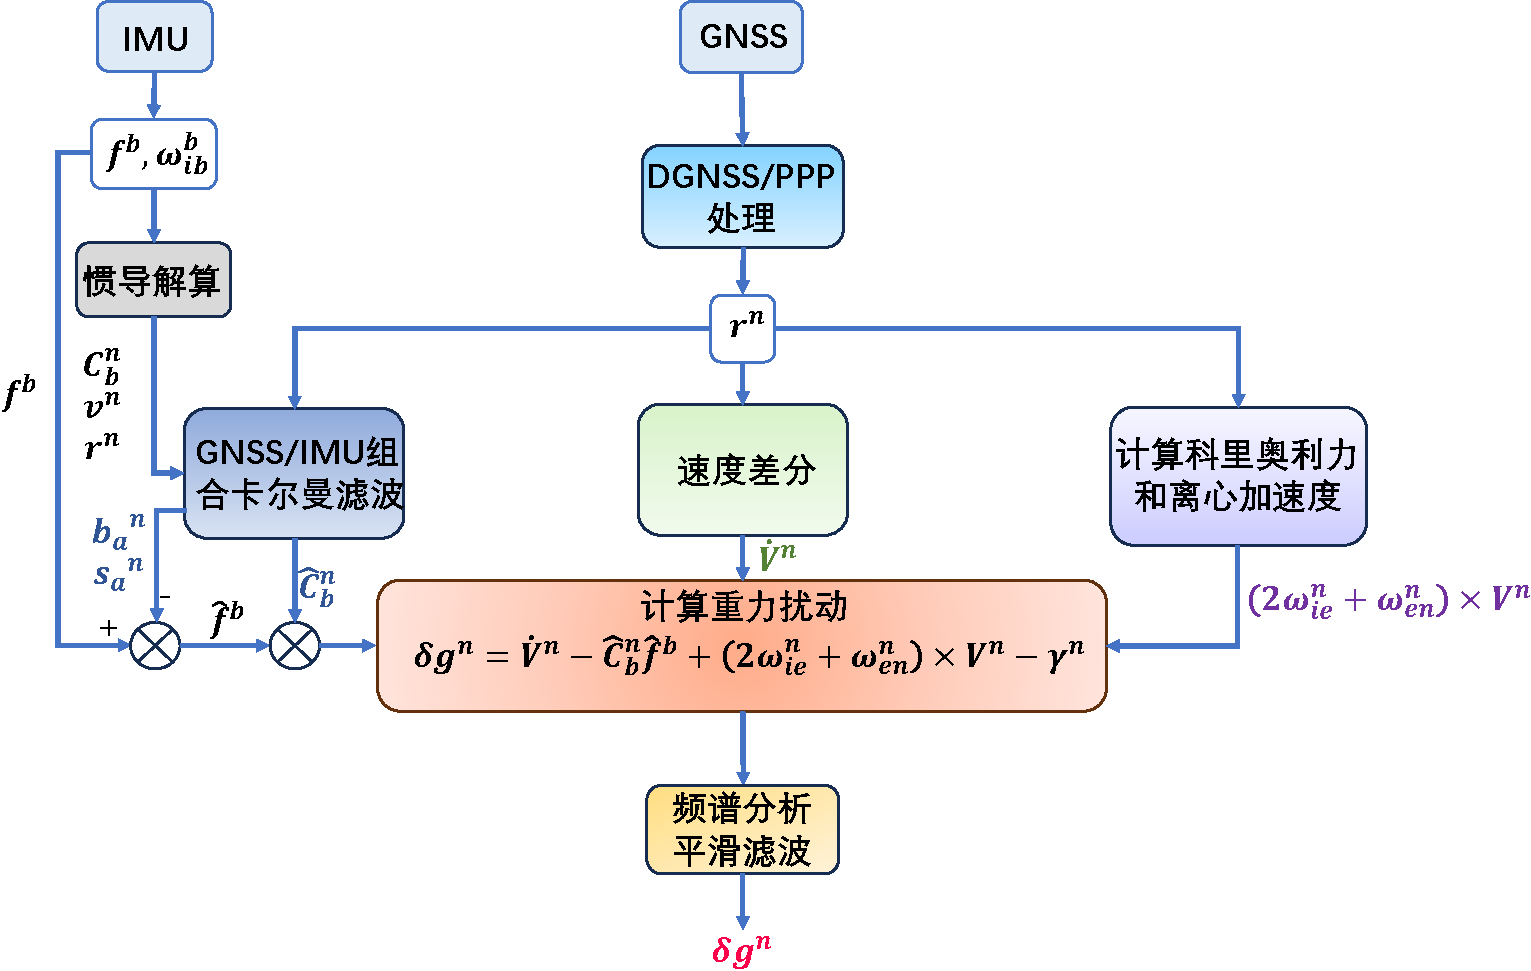
\includegraphics[width=0.8\textwidth]{figure/direct-crop.pdf}
      \captionsetup{font={footnotesize}}
      \caption{\label{fig:direct}直接测量}
\end{figure}

间接测量就相对比较复杂,如图\ref{fig:indirect}所示,它是基于构建的惯性导航参数误差的卡尔曼滤波器而间接得到的。除了姿态误差、速度误差、位置误差和传感器误差之外,额外增加了重力扰动的矢量误差$\bm{[\delta g^n]}$项,其具体的维数与模型构建的方式有关。由于IMU测量得到的位置是通过对其输出进行积分,那么包含重力重力扰动在内的误差值就可以从观测到的位置差异中估计出来。然而这种方法在构建卡尔曼状态方程时,最好能够将其与其它误差源进行区分,使其不相互影响。常见的方法是将其构建为高斯-马尔可夫模型\upcite{jekeli1994airborne,jordan1972self}和自回归模型(AR)\upcite{bruton2000improving,nassar2004modeling}。
\begin{figure}[h]
      \centering
      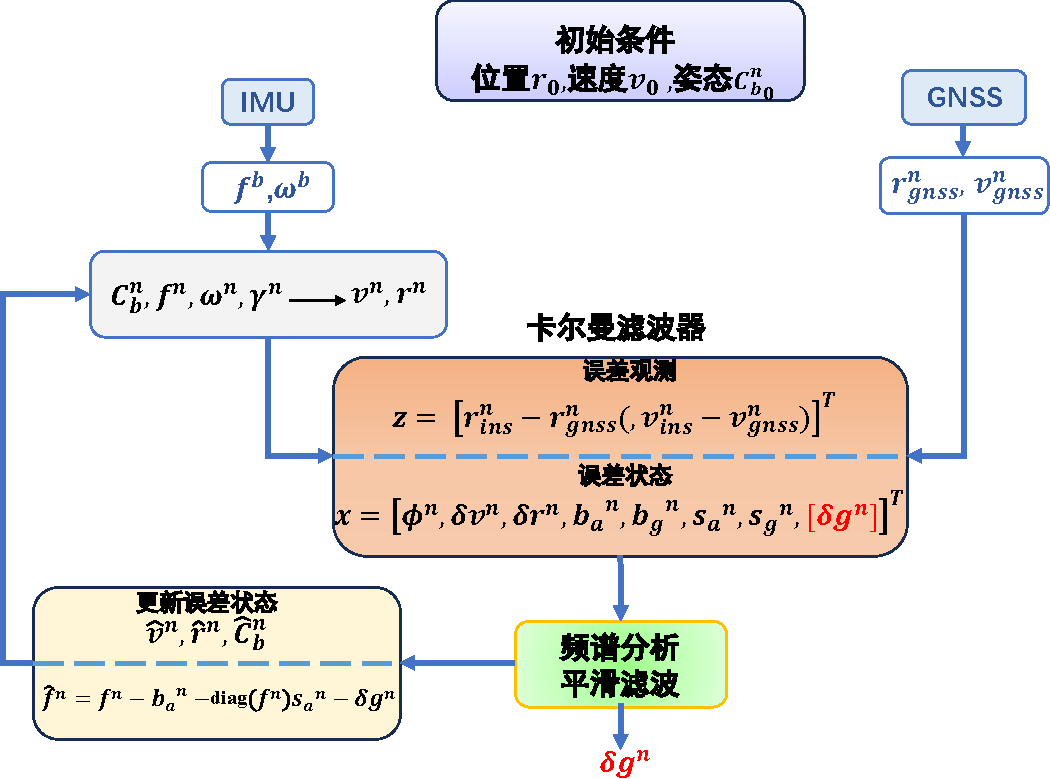
\includegraphics[width=0.8\textwidth]{figure/indirect-crop.pdf}
      \captionsetup{font={footnotesize}}
      \caption{\label{fig:indirect}间接测量}
\end{figure}
间接测量相比于直接测量,由于采用卡尔曼滤波器,其积分形式相比于直接测量的微分形式来说,数值上更稳定;但是同时,间接测量的方法极其依赖于其构建的模型,如果构建的模型不够准确,那么很难将有效的重力扰动从频谱中进行分离;并且如果采用低通滤波对测量数据进行处理,反而会失去一部分重力场的短波信息\upcite{schwarz1997introduction};更重要的是,由于使用卡尔曼滤波器对重力扰动估计需要先验值,那么最终估计得到的结果将会受限于先验假设的影响。但是相比之下,采用直接法则简单高效,更容易应用于GNSS/IMU集成的软件之上\upcite{jekeli2023inertial}。

\section{重力扰动对惯导解算的误差影响}
美军早在20世纪50年代末就已经开启重力辅助惯导技术研究,为了减弱惯导系统的舒勒振荡误差影响,当时主要聚焦于实现惯导系统力学编排中的扰动重力矢量参数(特别是垂线偏差)精确补偿。黄谟涛等人提出\upcite{WHCH20240724001},将重力辅助惯性导航技术划分为重力补偿和重力修正两个发展阶段,其中重力补偿技术是指在惯导解算回路中加入重力扰动信息以改善惯导系统的力学编排,达到抑制误差发散的趋势。下面我们将围绕重力扰动对惯导解算过程的影响机理进行分析。

\subsection{重力扰动的误差模型}
在惯性导航中,我们常常通过构建位置、速度和姿态误差的微分方程来描述误差源随时间传播的规律。根据第3节描述的重力扰动模型,在惯导解算的速度微分方程中,有
\begin{equation}
      \bm{\delta g^n} = \dot{\bm{v}^n}-\bm{C}^n_b\bm{f}^b+(2\bm{w}^n_{ie}+\bm{w}^n_{en})\times \bm{v}^n- \bm{\gamma}^n
      \label{equ_delta_g}
\end{equation}
在北-东-地坐标系下,可以得到其分量表示:
\begin{equation}
      \left\{ \begin{aligned}
      & \delta {{g}_{N}}={{{\dot{v}}}_{N}}-{{f}_{N}}+(2{{w}_{ie}}\sin L+\frac{{{v}_{E}}\tan L}{{{R}_{N}}+h}){{v}_{E}}-\frac{{{v}_{N}}{{v}_{D}}}{{{R}_{M}}+h} \\ 
      & \delta {{g}_{E}}={{{\dot{v}}}_{E}}-{{f}_{E}}-(\frac{{{v}_{E}}}{{{R}_{N}}+h}+2{{w}_{ie}}\cos L)({{v}_{D}}+{{v}_{N}}\tan L) \\ 
      & \delta {{g}_{D}}={{{\dot{v}}}_{D}}-{{f}_{D}}+(2{{w}_{ie}}\cos L+\frac{{{v}_{E}}}{{{R}_{N}}+h}){{v}_{E}}+\frac{v_{N}^{2}}{{{R}_{M}}+h}-\gamma  \\ 
\end{aligned} \right.
\label{equ_delta_g_more}
\end{equation}
其中,$R_N$和$R_M$分别表示卯酉圈半径和子午圈半径,$L$代表纬度,$w_{ie}$表示地球自转角速度。

于是,由式\ref{equ_delta_g}可以进一步得到重力扰动的误差模型,
\begin{equation}
      \begin{aligned}
      \text{d}\bm{\delta g}^n = &\bm{\delta} \dot{\bm{v}}^n + \bm{[\phi^n\times]}\bm{C}^n_b \bm{f}^b - \bm{C}^n_b \bm{\delta f}^b + 
      \\
      &(2\bm{\delta w}^n_{ie} +\bm{\delta w}^n_{en})\bm{\times v}^n+(2\bm{w}^n_{ie} + \bm{w}^n_{en})\bm{\times \delta v}^n - \bm{\delta \gamma}^n
      \end{aligned}
      \label{equ_diff_disturb}
\end{equation}
其中,$\text{d}\bm{\delta g}^n$代表重力扰动的误差,$\bm{[\phi^n \times]}$是姿态误差$\bm{\phi^n}$的反对称矩阵,$\bm{\delta \gamma}^n$代表正常重力的模型误差。

进一步的,当考虑惯性导航系统和卫星导航系统存在同步时间差$\text{d}T$时\upcite{schwarz1995some},式\ref{equ_diff_disturb}可以重新写作
\begin{equation}
      \begin{aligned}
      \text{d}\bm{\delta g}^n = &\bm{\delta} \dot{\bm{v}}^n + \bm{[\phi^n\times]}\bm{C}^n_b \bm{f}^b - \bm{C}^n_b \bm{\delta f}^b + (2\bm{\delta w}^n_{ie} + \bm{\delta w}^n_{en})\bm{\times v}^n
      \\
      &+\ddot{\bm{v}}^n\text{d}T+(2\bm{w}^n_{ie} + \bm{w}^n_{en})\bm{\times \delta v}^n - \bm{\delta \gamma}^n
      \end{aligned}
      \label{equ_diff_disturb_more}
\end{equation}

随着实时运动学差分GNSS技术的不断改进,采用实时运动学差分GNSS技术的定位精度和速度精度分别小于0.01m和0.03m/s。根据前面的分析,在式\ref{equ_diff_disturb}中由差分GNSS引起的最后三项误差均低于1mGal;当时间同步误差限制在50$\mu s$时,由同步时间差引起的$\ddot{\bm{v}}^n\text{d}T$误差项可维持在1mGal以内\upcite{hao2024methods}。因此,捷联式重力扰动的误差主要由动态加速度误差$\bm{\delta} \dot{\bm{v}}^n$、姿态误差$\bm{[\phi^n\times]}\bm{C}^n_b \bm{f}^b$和比力误差$\bm{C}^n_b \bm{\delta f}^b$引起的。

\subsection{对姿态的影响}


\subsection{对比力测量的影响}


\subsection{对初始对准的影响}


\subsection{对载体运动的影响}

\section{现有的补偿方法及策略}

\section{总结与展望}


\newpage
\subsection{致谢}
感谢博客园博主\href{https://www.cnblogs.com/huangliu1111/p/13625826.html}{@望舒}提供的部分代码参考,开源促进世界进步!
\subsection{联系作者}
作者QQ邮箱\href{https://wx.mail.qq.com/?cancel_login=true&from=get_ticket_fail}{1141470651@qq.com},欢迎进行讨论交流$(>\text{w}<)$,good luck!。

\bibliography{sample}

\end{document}